\documentclass{article}

\usepackage{fullpage,amsmath,amsthm,graphicx,enumitem}
\usepackage{hyperref}
\usepackage{amssymb}
\usepackage{wasysym}
\usepackage{empheq}
\usepackage{booktabs}
\usepackage{xfrac}
\usepackage{multicol}

%For Grid, thanks internet: https://tex.stackexchange.com/questions/247541/help-with-grid-lines-in-a-pgfplot
\usepackage{tikz}
\usepackage{pgfplots}
\usetikzlibrary{calc}

\theoremstyle{definition}
\newtheorem{question}{Question}

\title{ASEN 3728 Aircraft Dynamics\\Written Homework 8}

\date{Due date listed on Gradescope.}

\begin{document}

\maketitle

\begin{question}
    TRUE or FALSE and Justify:
    \begin{enumerate}[label=\alph*)]
        \item Improving the damping ratio of the spiral mode is a major design objective of lateral stability augmentation system design.

        \item Near trim for straight and level airplane flight, the rate of change in bank angle at time $t$ depends on the bank angle at time $t$.

        \item Near trim for straight and level airplane flight, the rate of change in the roll moment at time $t$ generally depends on the change in sideslip angle at time $t$.
    \end{enumerate}
\end{question}

\clearpage

\begin{question}
    A quadplane (pictured below) is an aircraft that combines features of a quadcopter and an airplane. 
\begin{center}
    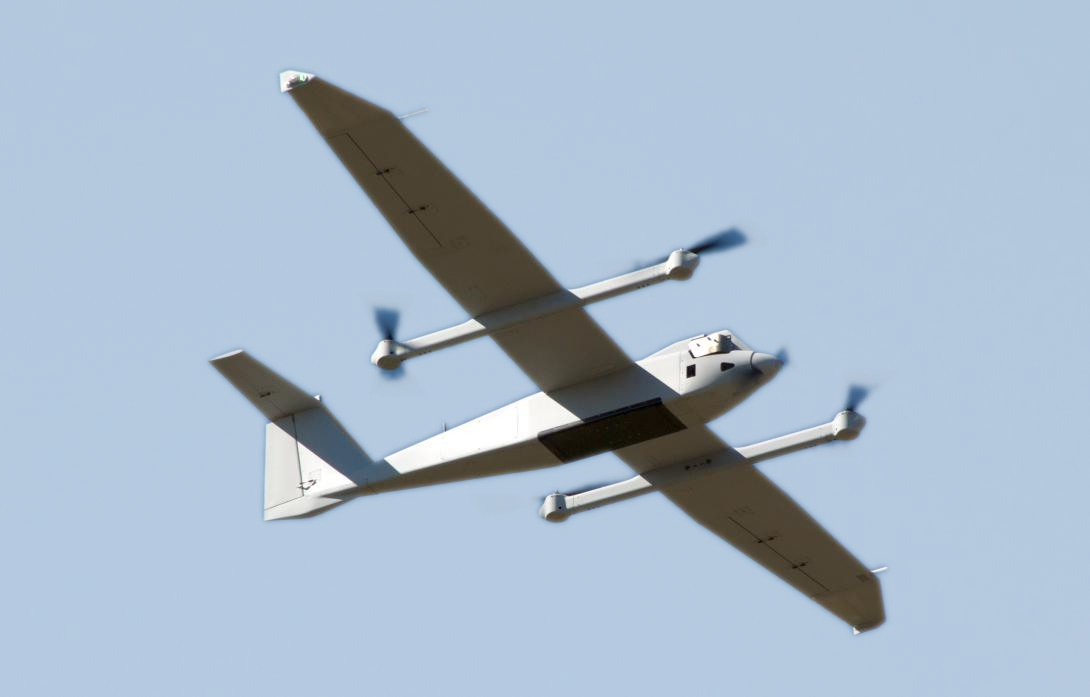
\includegraphics[width=0.25\textwidth]{figures/real-quadplane.png}
    \hspace{1cm}
    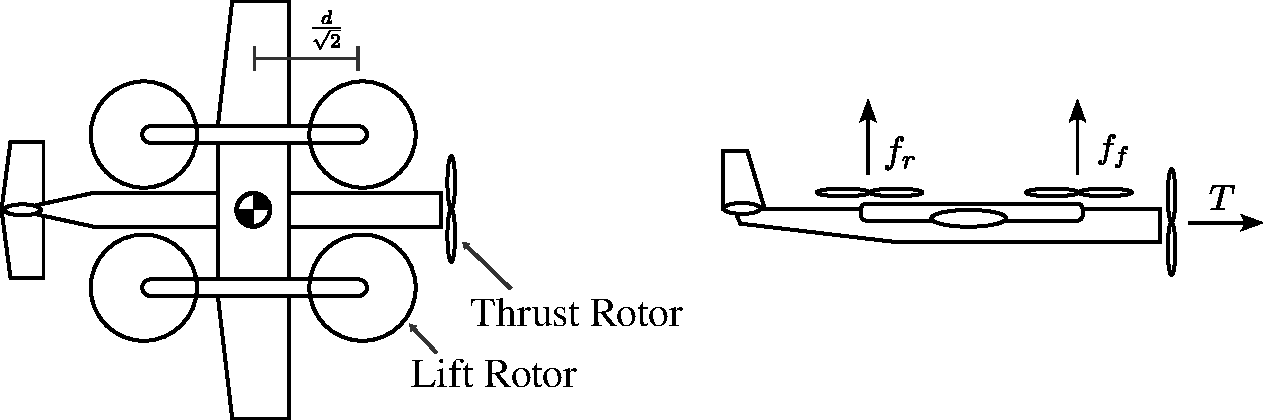
\includegraphics[width=0.5\textwidth]{figures/quadplane.pdf}\\
    Photo (left), overhead schematic (center), and side schematic (right) of a quadplane.
\end{center}

In slow forward flight, lift is generated by both the wings and the lift rotors. In this problem $f_f$ will denote the combined force generated by the front two rotors, and $f_r$ the combined force of the two rear rotors. For this problem, you may ignore aerodynamic interaction between the rotor wash and the wings, fuselage or other aerodynamic surfaces and any aeroelastic effects.
Some parameters for the aircraft are given below:
\begin{multicols}{3}
\begin{itemize}[nosep,label={}]
    \item $m = 6 \,kg$
    \item $K = 0.6 \text{ (induced drag parameter)}$
    \item $\rho = 1 \,kg/m^3$
    \item $S = 0.63 \,m^2$
    \item $C_{D_\text{min}} = 0.024$
    \item $C_{L_\text{min}} = 0$
    \item $d = 0.5\, m$
    \item $I_y = 0.9\, kg\, m^2$
    \item $C_{L_\alpha} = 6.2$
    \item $C_{m_\alpha} = -1.6$
    \item $C_{L_q} = 10$
    \item $C_{m_q} = -24$
    \item $C_{L_{\delta_e}} = 0.0068$
    \item $C_{m_{\delta_e}} = -0.06$
\end{itemize}
\end{multicols}

\begin{enumerate}[label=\alph*)]
    \item Assuming that thrust is opposite drag, and the forces associated with the lift rotors $f_f$ and $f_r$ are vertical,
        calculate $C_{L_0}$, $C_{D_0}$ and $T_0$ needed to maintain level flight at $V = 10 m/s$ with $f_f = f_r = 10N$.

    \item The following nonlinear equations can be used to approximate the phugoid mode for the quadplane:
        $$\dot{u} = \frac{1}{m}\left(-m g \sin \theta + T_0 - \frac{1}{2} \rho u^2 S C_{D_0}\right) \qquad \qquad \dot{\theta} = \frac{1}{m u_0} \left(\frac{1}{2} \rho u^2 S C_{L_0} + f_f + f_r\right) \text{.}$$
        If $\theta_0$ is defined to be $0$, linearize the above equations to find a symbolic $A$ matrix for a 2-dimensional state space system approximating the phugoid mode with state $[\Delta u, \Delta \theta]^T$.

    \item According the approximation derived above, in which of the following cases will the phugoid mode have a higher natural frequency: (a) flying near trim with the lift rotors turned off or (b) flying near trim with $f_f = f_r = 10N$?

    \item Ignoring unsteady effects ($\dot{w}$ derivatives) and assuming $\theta_0=0$, a linear longitudinal model for a conventional aircraft in straight and level flight is:
        \begin{equation}
            \begin{bmatrix} \dot{\Delta u} \\ \dot{\Delta w} \\ \dot{\Delta q} \\ \dot{\Delta \theta} \\ \end{bmatrix}
            = \begin{bmatrix}
                \sfrac{X_u}{m} & \sfrac{X_w}{m} & 0 & -g \\
                \sfrac{Z_u}{m} & \sfrac{Z_w}{m} & \sfrac{(Z_q + m u_0)}{m} & 0 \\
                \sfrac{M_u}{I_y} & \sfrac{M_w}{I_y} & \sfrac{M_q}{I_y} & 0 \\
                0 & 0 & 1 & 0 \\
            \end{bmatrix}
            \begin{bmatrix} \Delta u \\ \Delta w \\ \Delta q \\ \Delta \theta \end{bmatrix}
            + \begin{bmatrix}
                \sfrac{(\Delta T + X_{\delta_e} \Delta \delta_e)}{m} \\
                \sfrac{Z_{\delta_e} \Delta \delta_e}{m} \\
                \sfrac{M_{\delta_e} \Delta \delta_e}{I_y} \\
                0
            \end{bmatrix}
        \end{equation}

        while a similar linear model for a quadrotor near hover is:
        \begin{equation}
            \begin{bmatrix} \dot{\Delta u} \\ \dot{\Delta w} \\ \dot{\Delta q} \\ \dot{\Delta \theta} \end{bmatrix}
            = \begin{bmatrix} 
                0 & 0 & 0 & -g \\
                0 & 0 & 0 & 0  \\
                0 & 0 & 0 & 0  \\
                0 & 0 & 1 & 0  \\
            \end{bmatrix}
            \begin{bmatrix} \Delta u \\ \Delta w \\ \Delta q \\ \Delta \theta \end{bmatrix}
            + \begin{bmatrix}
                0 \\
                -\sfrac{1}{m} (\Delta f_f + \Delta f_r) \\
                \sfrac{d}{(\sqrt{2} I_y)} (\Delta f_f - \Delta f_r) \\
                0 \\
            \end{bmatrix}
        \end{equation}

        where $\Delta f_f = f_f - f_{f_0}$ and $\Delta f_r = f_r - f_{r_0}$ and $f_{f_0}$ and $f_{r_0}$ are the lift rotor thrusts at hover.

        What is the analogous linear model for the quadplane at a \textbf{hover} trim condition? Clearly justify your answer using equations or words. Where possible, replace symbols with numerical values.
\end{enumerate}

\end{question}

\clearpage

\begin{question}
    Consider an aircraft with the following lateral $A$ and $B$ matrices for state vector $\mathbf{x} = [\Delta v,\Delta p,\Delta r,\Delta \phi]^T$ and control vector $\mathbf{u} = [\Delta \delta_a,\Delta \delta_r]^T$:
\begin{align*}
    A = 
    \begin{pmatrix}
        -0.4 & 0.5 & -21 & 9.8 \\
        -1.3 & -5.2 & 3.1 & 0 \\
        0.7 & -1.4 & -0.6 & 0 \\
        0 & 1 & 0.03 & 0
    \end{pmatrix} \quad \quad
    B = 
    \begin{pmatrix}
        -0.02 & 0.08 \\
        -2.50 & 0.04 \\
        -0.35 & -0.18 \\
        0 & 0
    \end{pmatrix}
\end{align*}

Suppose that you are designing a stability augmentation system (SAS) with a roll component that augments the pilot's aileron input, $\Delta \delta_{a, c}$ so that $\Delta \delta_a = -k_a \Delta p + \Delta \delta_{a,c}$ and a similar yaw component that yields $\Delta \delta_r = -k_r \Delta r + \Delta \delta_{r,c}$, where $\delta_{r,c}$ is the pilot's rudder input. The two root locus plots below show how the SAS modifies the poles of the system for different values of $k_a$ and $k_r$.

\begin{minipage}{0.5\textwidth}
    \begin{center}
        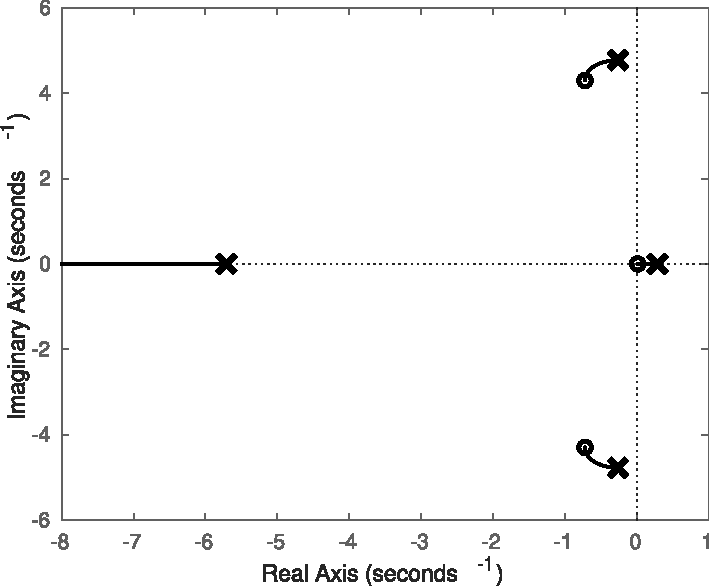
\includegraphics[height=6cm]{figures/roll_root_locus.pdf}\\
        Root locus for negative values of $k_a$
    \end{center}
\end{minipage}
\begin{minipage}{0.5\textwidth}
    \begin{center}
        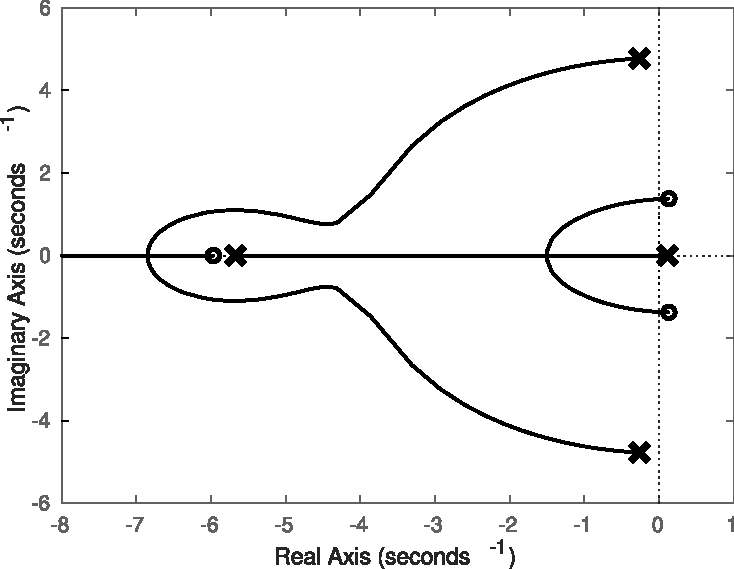
\includegraphics[height=6cm]{figures/yaw_root_locus.pdf}\\
        Root locus for negative values of $k_r$
    \end{center}
\end{minipage}

\begin{enumerate}[label=\alph*)]
    \item Which gain would be most useful for \textbf{increasing the damping ratio of the dutch roll mode}? Justify your answer with a brief explanation \textbf{and} by indicating the relevant part of the root locus plot by circling it \textbf{on your answer sheet} and writing ``Part 1'' near it.
    \item Which gain would be most useful for \textbf{decreasing the time constant of the roll mode}? Justify your answer with a brief explanation \textbf{and} by indicating the relevant part of the root locus plot by circling it \textbf{on your answer sheet} and writing ``Part 2'' near it.
    \item Which gain would be most useful for \textbf{stabilizing the spiral mode}? Justify your answer with a brief explanation \textbf{and} by indicating the relevant part of the root locus plot by circling it \textbf{on your answer sheet} and writing ``Part 3'' near it.
    % \item Under the pure roll mode approximation, the evolution of the roll rate depends on just one of the entries in $A$ and one of the entries in $B$. Write a symbolic equation for $\Delta \Dot{p}$ in terms of $\mathcal{L}_p$, $\mathcal{L}_{\delta_a}$, $\Delta p$, and $\Delta \delta_a$ for this mode approximation.
    \item Using the pure roll approximation ($\Delta \dot{p} = \mathcal{L}_p \Delta p + \mathcal{L}_{\delta_a} \Delta \delta_a$), derive a transfer function $G_{p\,\delta_a}(s)$ relating the aileron deflection to roll rate without the SAS. (Use numerical values rather than symbols in your final answer)
    \item Starting from trim, the pilot commands an aileron deflection of $\Delta \delta_a = -0.5$ rad to start a roll. What is the time derivative of the roll rate, $\Delta \Dot{p}$, at the instant the roll starts?
    \item Draw a block diagram showing the pure roll approximation and the aileron SAS control law above. The completed block diagram should have the pilot's commanded aileron ($\Delta \delta_{a,c}$) as the input and the roll rate ($\Delta p$) as the output. 
    \item Derive a closed-loop transfer function $G_{p\,\delta_{a,c}}(s)$ relating the commanded aileron deflection to roll rate with the SAS. Using the final value theorem, calculate the steady state roll rate if the pilot maintains the aileron deflection at $\Delta \delta_{a,c} = -0.5$ rad with the SAS gain $k_a = -0.3$.
   

    
    % After the pilot initiates the roll, the aileron deflection goes under closed loop control, with controller $\Delta \delta_a = -k_a \Delta p$. Substitute this $\Delta \delta_a$ into your equation from the previous part so that $\Delta \Dot{p}$ is in terms of $\mathcal{L}_p$, $\mathcal{L}_{\delta_a}$, $\Delta p$, and $k_a$.

    % \item At some point during the roll, $\Delta p = 0.75$ rad/s. If $k_a = -0.9$ and the closed loop control is active, what time interval is needed for the roll rate to decrease from 0.75 rad/s to 0.1 rad/s?
    % \item A calculation of the transfer function $G_{{\Delta p}_{\Delta \delta a}}(s)$ relating the aileron deflection to roll rate requires matrices $A$, $B$, and $C$ based off the definition in lecture. Write out the matrices you would use to find the transfer function. For $A$ and $B$, you can either re-write the numbers you need or indicate what part of the given lateral $\mathbf{A}$ and $\mathbf{B}$ matrices you would use. Also, don't assume any mode approximation for this part.
    
\end{enumerate}
\end{question}

\end{document}